\documentclass[12pt]{article}

\usepackage[T1]{fontenc}
\usepackage[polish]{babel}
\usepackage[utf8]{inputenc}
\usepackage{lmodern}
\selectlanguage{polish}

\usepackage{graphicx}
\usepackage{tabularx, booktabs}
\usepackage{fancyhdr} 
\usepackage{geometry}
\usepackage{hyperref}
\usepackage{listings}
\usepackage{float} 


\usepackage{a4wide}

\geometry{left=15mm,right=25mm,%
bindingoffset=10mm, top=20mm, bottom=20mm}
 


\renewcommand{\maketitle}{
\begin{titlepage}
\begin{table}[t]
\centering
\begin{tabular}[t]{lcr}
 
\includegraphics[width=70pt,height=70pt]{PW} & POLITECHNIKA WARSZAWSKA & 
\includegraphics[width=70pt,height=70pt]{MiNI}\\
& WYDZIAŁ MATEMATYKI & \\
& I NAUK INFORMACYJNYCH &
\end{tabular}
\end{table}
\vspace*{3cm}
  \begin{center}
    \LARGE
    \textbf {MSI2 - Raport}\\
   \vspace*{2 cm}
\begin{table}[!htp]
\begin{tabular}{p{4cm}p{9cm}}
\textit{Przedmiot:} &\textbf {Metody sztucznej inteligencji 2} \\
\\
\textit{Projekt:} &\textbf {Agent do grania w gry Atari przy użyciu uczenia wzmocnionego (reinforcement learning)} \\
\\
\textit{Autorzy:} &\textbf {Michał~Kołodziej \newline Nikodem~Wiśniewski} \\
\\
\end{tabular}
\end{table}

\vspace{5 cm}
  \center{\small Warszawa, dnia \today}
\end{center}
\end{titlepage}
}

\begin{document}
\maketitle


\section{Opis projektu}
Zadaniem tego projektu jest stworzenie agenta komputerowego grającego w gry z Atari 2600. Agent jest trenowany za pomocą uczenia przez wzmacnianie (reinforcement learning) poprzez samoczynne granie w wybrane gry. Agent miał styczność z wieloma grami z konsoli Atari.

\section{Metodyka}

Podczas uczenia agent ma przedstawione jako stan 4 ostatnie klatki z gry. Dzięki temu ma on nie tylko podgląd obecnego ekranu ale również widzi on zmiany w grze. W celu ograniczenia ilości przetwarzanych danych ograniczymy rozmiar klatki do 86x86 pikseli w 256 wymiarowej skali szarości.
\\\

\subsection{Nagrody}

Na poączątku zdefiniujmy pojęcie nagrody w kontekście nauczania ze wzmocnieniem. Agent za każdą akcję dostaję nagrodę, agent dąży do maksymalizacji nagród w trakcie jednej gry. W naszym przypadku nagroda będzie wynosiła 0 lub 1. Końcowy wynik agenta możemy określić jako sumę nagród po wykonaniu n akcji:

$$R=r_1 + r_2 + r_3 + \dots + r_n$$

Na tej podstawie jesteśmy w stanie zdefiniować równanie do uzyskania sumę nagród w przyszłości:

$$R_t=r_t + r_{t+1}+ r_{t+2} + \dots + r_n$$

Niestety w naszym środowisku niektóre zachowania gier są losowe przez co musimy zaburzyć tą sumę zmniejszając nagrody odsunięte dalej w przyszłości gdyż są one mniej pewne niż nagroda za kolejny krok agenta. Korzystamy wówczas z równania na sumę nagród z \textit{rabatem}:

$$R_t=r_t + \gamma r_{t+1}+  \gamma^2 r_{t+2} + \dots + \gamma^{n-t}r_n$$

W sumie z \textit{rabatem} nagrody są pomniejszane o czynnik $\gamma$ który jest liczbą z przedziału $[0,1]$ gdzie dla $\gamma =0$ strategia jest krótkoterminowa i patrzymy tylko na najbliższą nagrodę, zaś dla $\gamma =1$ zakładamy iż środowisko jest deterministyczne i kolejne akcje zawsze wywołują te same stany.

\subsection{Q-learning}

Do wyliczania kolejnych ruchów agenta skorzystaliśmy z \textbf{Q-learningu}. Zdefiniujmy funkcję \textit{Q(s,a)} gdzie \textit{s} to stan, zaś \textit{a} to akcja możliwa do wykonania w danym stanie. Funkcja ta reprezentuje możliwie największy wynik pod koniec gry w przypadku podjęcia akcji \textbf{a} w stanie \textbf{s}. Jest ona określona rekurencyjnym równaniem Bellmana:

$$Q(s,a) =  r + \gamma max_{a'}Q(s',a')$$

Gdzie $r$ to nagroda po wykonaniu akcji $a$ w stanie $s$, $\gamma$ to współczynnik rabatu, $s'$ to stan w którym znajdziemy się po wykonaniu akcji $a$, zaś $a'$ to kolejna akcja.

\subsection{Deep Q Network}

W związku z tym że każda z 4 ostatnich klatek gry ma rozdzielczość $8x\times 84$, a każdy piksel może mieć 256 możliwych wartości w skali szarości wówczas mamy $256^{84\times84\times4}$ stanów gry. Jest to tak ogromna liczba iż nie jesteśmy w stanie stworzyć tablicy zapamiętania funkcji Q.
Aby skutecznie liczyć wartość funkcji $Q(s,a)$ naszym projekcie skorzystaliśmy z sieci neuronowej do tego zadania. Nasza sieć na wejściu przyjmuje stan gry (4 klatki z gry), a na wyjściu daje nam wartość funkcji Q dla każdej możliwej akcji. W Atari 2600 mamy do wykonania 18 możliwych akcji (chociaż nie wszystkie są używane we wszystkich grach).
\\\

Dla przejścia $<s, a, r, s'>$ aktualizujemy naszą sieć następującym algorytmem:
\begin{enumerate}
\item Wykonujemy feedforward dla obecnego stanu $s$ aby uzyskać przewidywane Q-wartości dla każdej akcji. Oznaczmy wyliczone w ten sposób wartości $Q'(s,a)$.
\item Wykonujemy feedforward dla kolejnego stanu $s'$ i wybieramy wartość dla najlepszej akcji $max_{a'}Q(s',a')$.
\item Wyliczamy poprawną wartość funkcji $Q$ dla akcji $a$ korzystając ze wzoru: $$Q(s, a) = r + max_{a'}Q(s',a')$$ Dla innych akcji zostawiamy wartość funkcji $Q$ uzyskaną z naszej sieci.
\item Liczymy funkcję straty (loss function) wzorem $$L=\frac{1}{2}[Q(s,a)-Q'(s,a)]^2=\frac{1}{2}[r+\gamma max_{a'}Q(s',a')-Q'(s,a)]^2$$ Uwaga: funkcja straty dla akcji innych niż $a$ przez powyższe założenie wynosi 0. 
\item Aktualizujemy wagi w sieci używając backpropagation
\end{enumerate}

\subsubsection{Experience replay}

W trakcie gry wszystkie doświadczenia <s, a, r, s'> zapisujemy w pamięci. Przy trenowaniu sieci losowe próbki są używane zamiast ostatnich przejść. W ten sposób łamiemy podobieństwo kolejnych trenujących gier, które mogą doprowadzać do minimów lokalnych w sieci.

\subsubsection{Exploration-exploitation dilemma}

Podczas inicjalizacji nasza sieć jest wypełniania losowymi liczbami więc początkowo wybierane akcje również będą losowe. Jest to czysta eksploracja. W przypadku gdy nasza sieć zbiega się do niektórych rozwiązań nasz algorytm nie będzie przeszukiwał nowych ścieżek i zachowań. Aby temu zapobiec skorzystamy z $\varepsilon\ greedy\ exploration$ z prawdopodobieństwem $\varepsilon$ na wykokanie losowej akcji. W oryginalnym projekcie firmy DeepMind wykorzystano zmienne w czasie $\varepsilon$ malejące od 1 do 0.1.

\subsubsection{Algorytm trenowania}

\begin{lstlisting}
 zainicjalizuj pamiec doswiadczen replay D
 zainicjalizuj siec neuronowa losowymi wagami
 pobierz stan s
 dopoki gra sie nie zakonczyla
	wybierz akcje a
		z prawdopodobienstwem $\varepsilon$ wybierz losowa akcje
		w przeciwnym przypadku wybierz $a = argmax_{a'}Q(s,a')$
	wykonaj akcje a
	pobierz nagrode r oraz stan s'
	zapisz doswiadczenie <s,a,r,s'> w pamieci D
	
	probkuj losowe przejscie <ss, aa, rr, ss'> z pamieci doswiadczen replay D
	oblicz dla kazdej miniporcji przejsc
		jezeli ss' jest stanem koncowym wowczas $tt=rr$
		w przeciwnym przypadku $tt=rr+\gamma argmax_{aa'}Q(ss', aa')$
	trenuj siec neuronowa uzywajac funkcji straty $tt-Q(ss,aa))^2$
	
	s=s'

\end{lstlisting}

\begin{figure}[H]
\centering 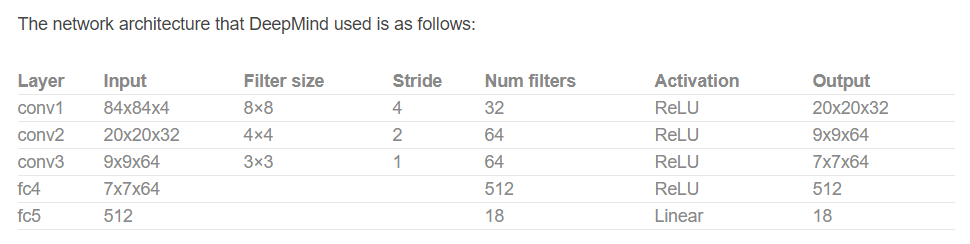
\includegraphics[scale=0.7]{deep_mind_architecture.PNG}
\caption{Sieć neuronowa firmy Deep Mind}
\label{simple1}
\end{figure}


\end{document}